\documentclass{beamer}

% Load packages
\usepackage[utf8]{inputenc}
\usepackage[pdf]{graphviz}

% Look and feel
\usetheme{metropolis}

% Title
\title[The RITAS algorithm]{The RITAS algorithm}
\subtitle{A constructive yield monitor data processing algorithm}
\author[Damiano, Niemi]{Luis Damiano}
\date{2020-10-23}
\institute[ISU]{Department of Statistics\\Iowa State University}

%%%%%%%%%%%%%%%%%%%%%%%%%%%%%%%%%%%%%%%%%%%%%%%%%%%%%%%%%%%%%%%%%%%%%%%%%%
% Document                                                               %
%%%%%%%%%%%%%%%%%%%%%%%%%%%%%%%%%%%%%%%%%%%%%%%%%%%%%%%%%%%%%%%%%%%%%%%%%%
\begin{document}

\begin{frame}
  \maketitle

  {\footnotesize
    Funded, in part, by
    \begin{itemize}
    \item[-] the Iowa State University Presidential Interdisciplinary
      Research Initiative on C-CHANGE: Science for a Changing Agriculture
    \item[-] Foundation for Food and Agriculture Research.
    \end{itemize}
  }
\end{frame}

\begin{frame}
  
  \frametitle{Road map}
  \tableofcontents
  
\end{frame}

%%%%%%%%%%%%%%%%%%%%%%%%%%%%%%%%%%%%%%%%%%%%%%%%%%%%%%%%%%%%%%%%%%%%%%%%%%
% Intro                                                                  %
%%%%%%%%%%%%%%%%%%%%%%%%%%%%%%%%%%%%%%%%%%%%%%%%%%%%%%%%%%%%%%%%%%%%%%%%%%

\section{Introduction}

\begin{frame}
  \frametitle{Context}

  % Worked on this first summer
  % The original STRIPS research question (link) needed a good way to
  % assign each observation to a treatment zone (show figure from
  % that report)
  
\end{frame}

\begin{frame}
  \frametitle{Sampling process}

  % Combine picture (internals)
  % GPS receiver picture
  
\end{frame}

\begin{frame}
  \frametitle{Uncertainty map}

  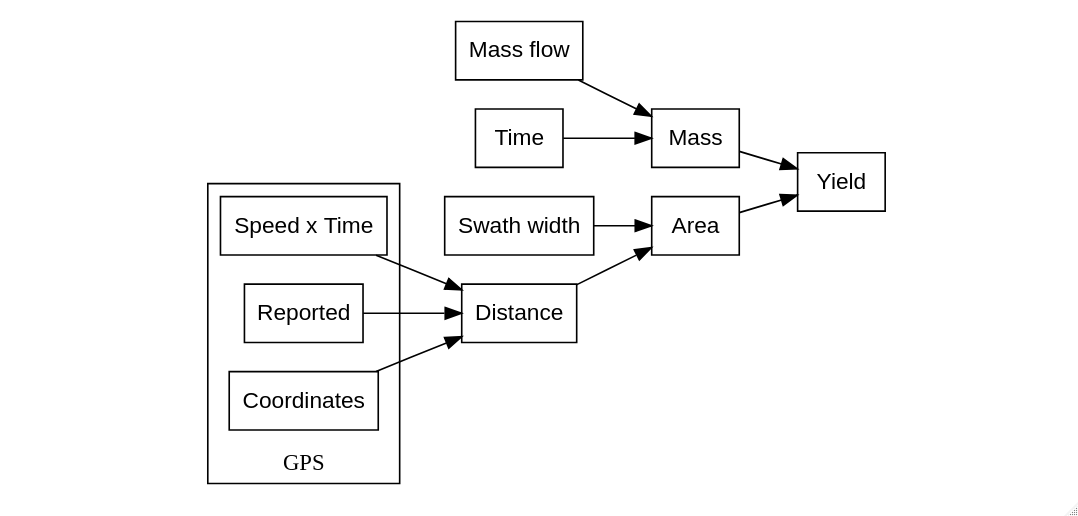
\includegraphics[width=0.95\textwidth]{./figures/uncertainty.png}
  
  % Uncertainty map
  %  Swath width (false constant), time & speed -> distance, mass,
  %  yield, time lag (different color)
  
\end{frame}

\begin{frame}
  \frametitle{Modeling challenges}

  % Show yield vs mass
  % histogram & semivariograms
  % Coefficient of variation
  % Extreme values
  % log yield vs log mass
  % Histogram of area (d * w)

\end{frame}

\begin{frame}
  \frametitle{Current analysis methodology}

  % Mention and point weaknesses
  
\end{frame}

%%%%%%%%%%%%%%%%%%%%%%%%%%%%%%%%%%%%%%%%%%%%%%%%%%%%%%%%%%%%%%%%%%%%%%%%%%
% The RITAS algo                                                         %
%%%%%%%%%%%%%%%%%%%%%%%%%%%%%%%%%%%%%%%%%%%%%%%%%%%%%%%%%%%%%%%%%%%%%%%%%%

\section{The RITAS algorithm}

\begin{frame}
  \frametitle{RITAS}

  \begin{columns}
    \begin{column}{0.30\textwidth}
      \begin{itemize}
      \item<1-> Rectangles
      \item<2-> Intersection
      \item<3-> Tessellation
      \item<4-> Apportioning
      \item<5-> Smoothing
      \end{itemize}
    \end{column}
    \begin{column}{0.70\textwidth}
      \begin{center}
        \includegraphics<1>[width=0.95\textwidth]{./figures/intro_rectangles}
        \includegraphics<2>[width=0.95\textwidth]{./figures/intro_intersection}
        \includegraphics<3>[width=0.95\textwidth]{./figures/intro_tessellation}
        \includegraphics<4>[width=0.95\textwidth]{./figures/intro_apportioning}
        \includegraphics<5>[width=0.95\textwidth]{./figures/intro_smoothing}
      \end{center}
    \end{column}
  \end{columns}
\end{frame}

%%%%%%%%%%%%%%%%%%%%%%%%%%%%%%%%%%%%%%%%%%%%%%%%%%%%%%%%%%%%%%%%%%%%%%%%%%
% STRIPS                                                                 %
%%%%%%%%%%%%%%%%%%%%%%%%%%%%%%%%%%%%%%%%%%%%%%%%%%%%%%%%%%%%%%%%%%%%%%%%%%

\section{STRIPS}

\begin{frame}
  \frametitle{Data set}

  % Description of the dataset
  
\end{frame}

\begin{frame}
  \frametitle{Results}

  % Maps -- maybe step by step
  % Gif

  \begin{center}
    \includegraphics<1>[width=0.95\textwidth]{./figures/maps_clipped/basswood_2012_01_points.png}
    \includegraphics<2>[width=0.95\textwidth]{./figures/maps_clipped/basswood_2012_02_rectangles.png}
    \includegraphics<3>[width=0.95\textwidth]{./figures/maps_clipped/basswood_2012_03_tessellation.png}
    \includegraphics<4>[width=0.95\textwidth]{./figures/maps_clipped/basswood_2012_04_chopped_res3_3.png}
    \includegraphics<5>[width=0.95\textwidth]{./figures/maps_clipped/basswood_2012_05_apportioned_res3_3.png}
    \includegraphics<6>[width=0.95\textwidth]{./figures/maps_clipped/basswood_2012_06_smoothed_res3_3.png}
  \end{center}
\end{frame}

%%%%%%%%%%%%%%%%%%%%%%%%%%%%%%%%%%%%%%%%%%%%%%%%%%%%%%%%%%%%%%%%%%%%%%%%%%
% Discussion                                                             %
%%%%%%%%%%%%%%%%%%%%%%%%%%%%%%%%%%%%%%%%%%%%%%%%%%%%%%%%%%%%%%%%%%%%%%%%%%

\section{Discussion}

\begin{frame}
  \frametitle{Pros and cons}

  % Compare with other work
  
\end{frame}

%%%%%%%%%%%%%%%%%%%%%%%%%%%%%%%%%%%%%%%%%%%%%%%%%%%%%%%%%%%%%%%%%%%%%%%%%%
% Future work                                                            %
%%%%%%%%%%%%%%%%%%%%%%%%%%%%%%%%%%%%%%%%%%%%%%%%%%%%%%%%%%%%%%%%%%%%%%%%%%

\section{Future work \\ \small{Preview}}

\begin{frame}
  \frametitle{Preview: color palette}

  % Palette
  % Colorblind & intuitive
  
\end{frame}

\begin{frame}
  \frametitle{Preview: absolute scale}

  % Absolute scale
  % Challenge: how to estimate the variance?
  
\end{frame}

\begin{frame}
  \frametitle{Preview: clipping}

  % Clipping (aesthetics)
  % Challenge: how to identify "boundaries"? inner voids?
  
\end{frame}

\begin{frame}
  \frametitle{Preview: rectangle scaling}

  % Rectangle scaling
  
\end{frame}

\section{Future work \\ \small{Where to start?}}

\begin{frame}
  \frametitle{Quantification}

  % How to quantify the smoothness.
  % How challenging is my dataset?
  % Show two rectangle plots
  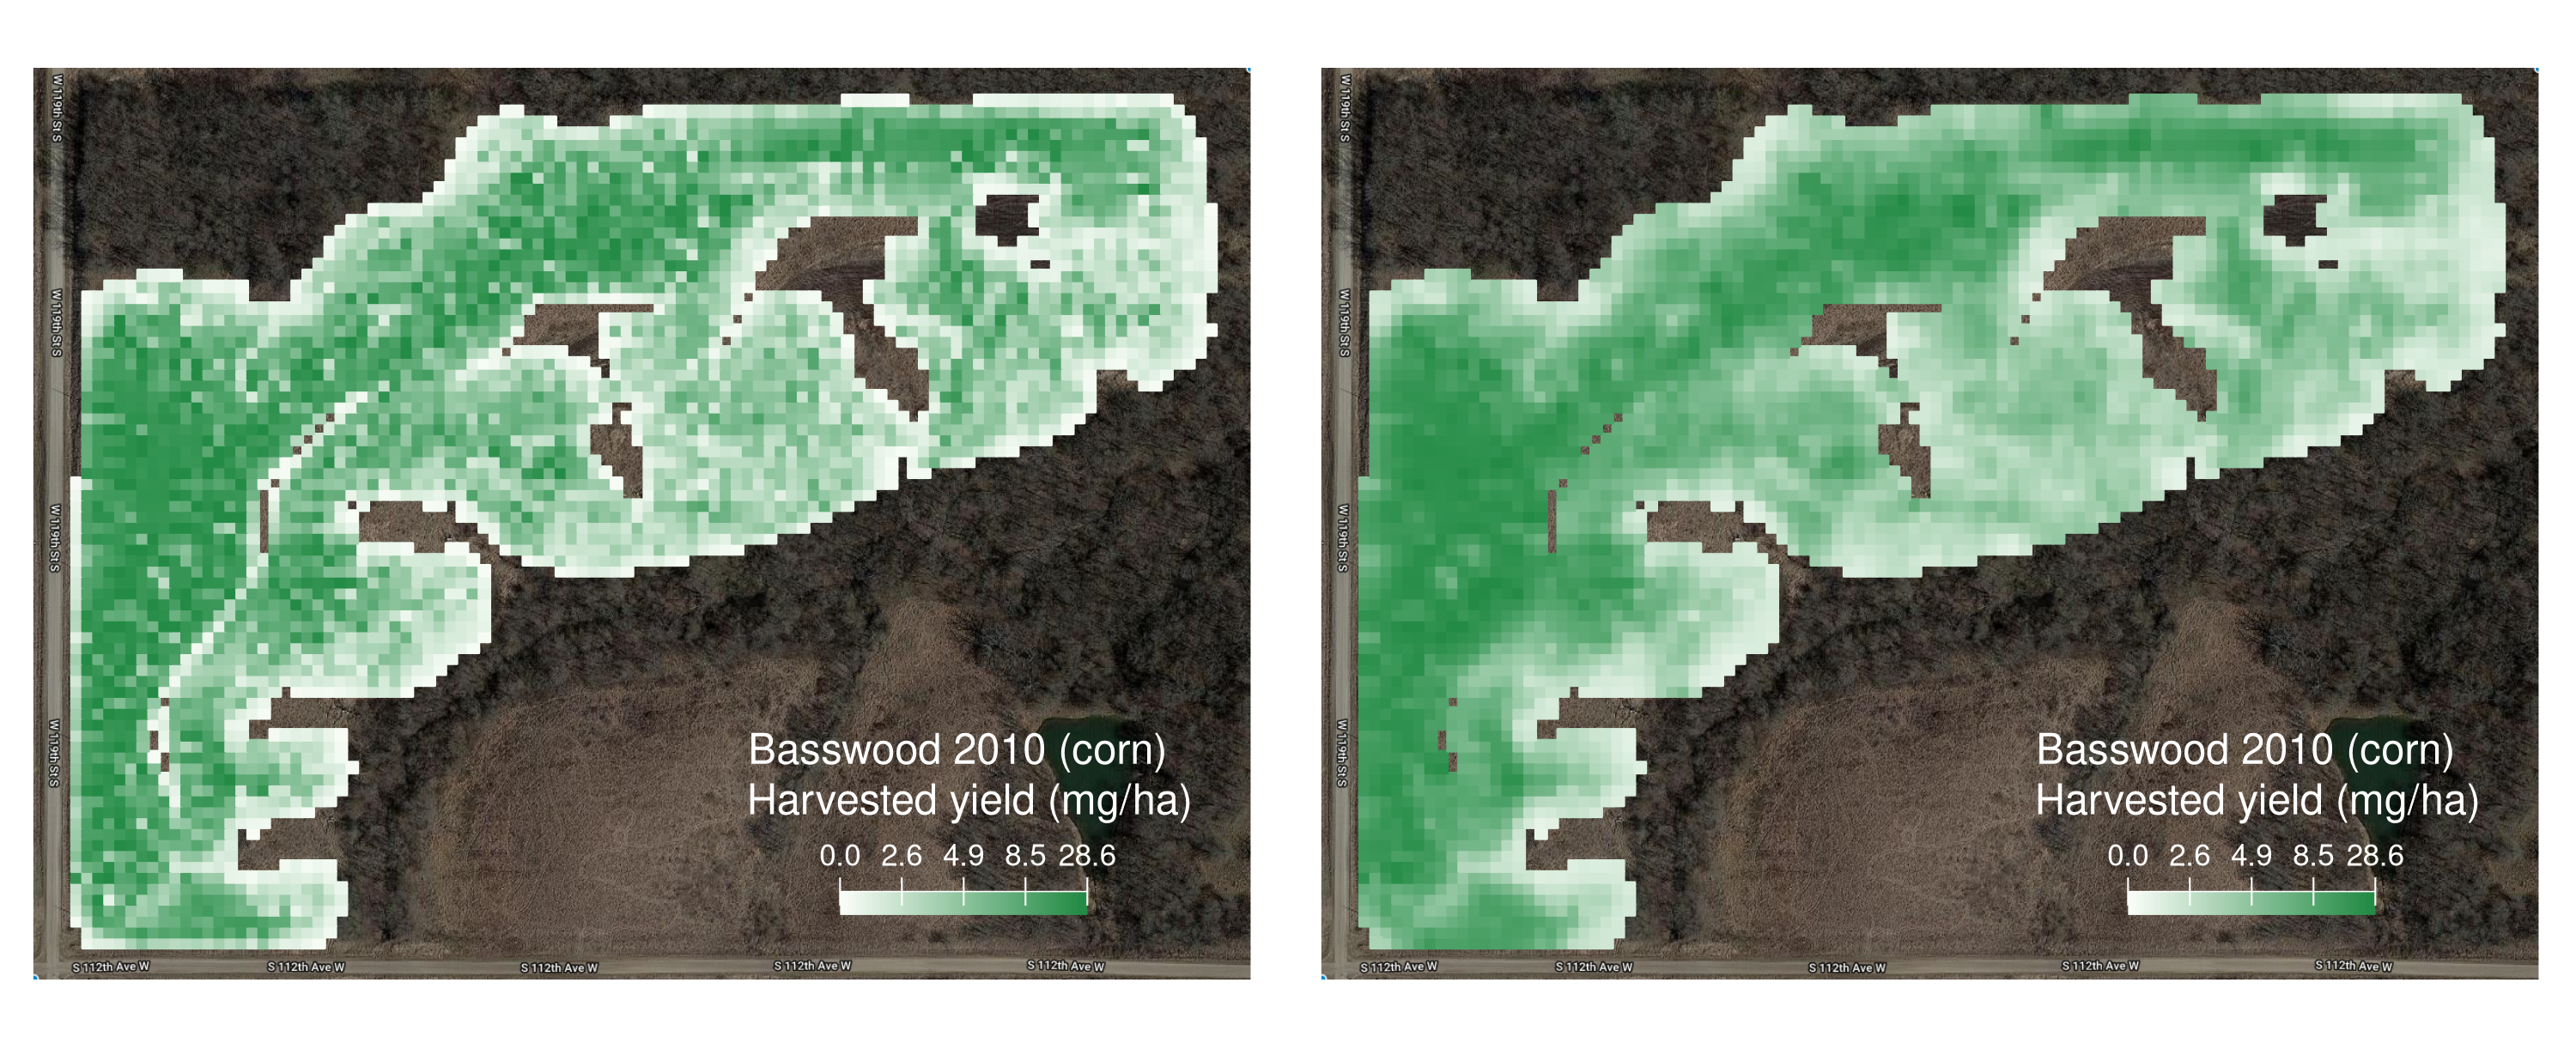
\includegraphics[width=0.95\textwidth]{./figures/maps/basswood_2010_07_gallery_res5_5.png}
  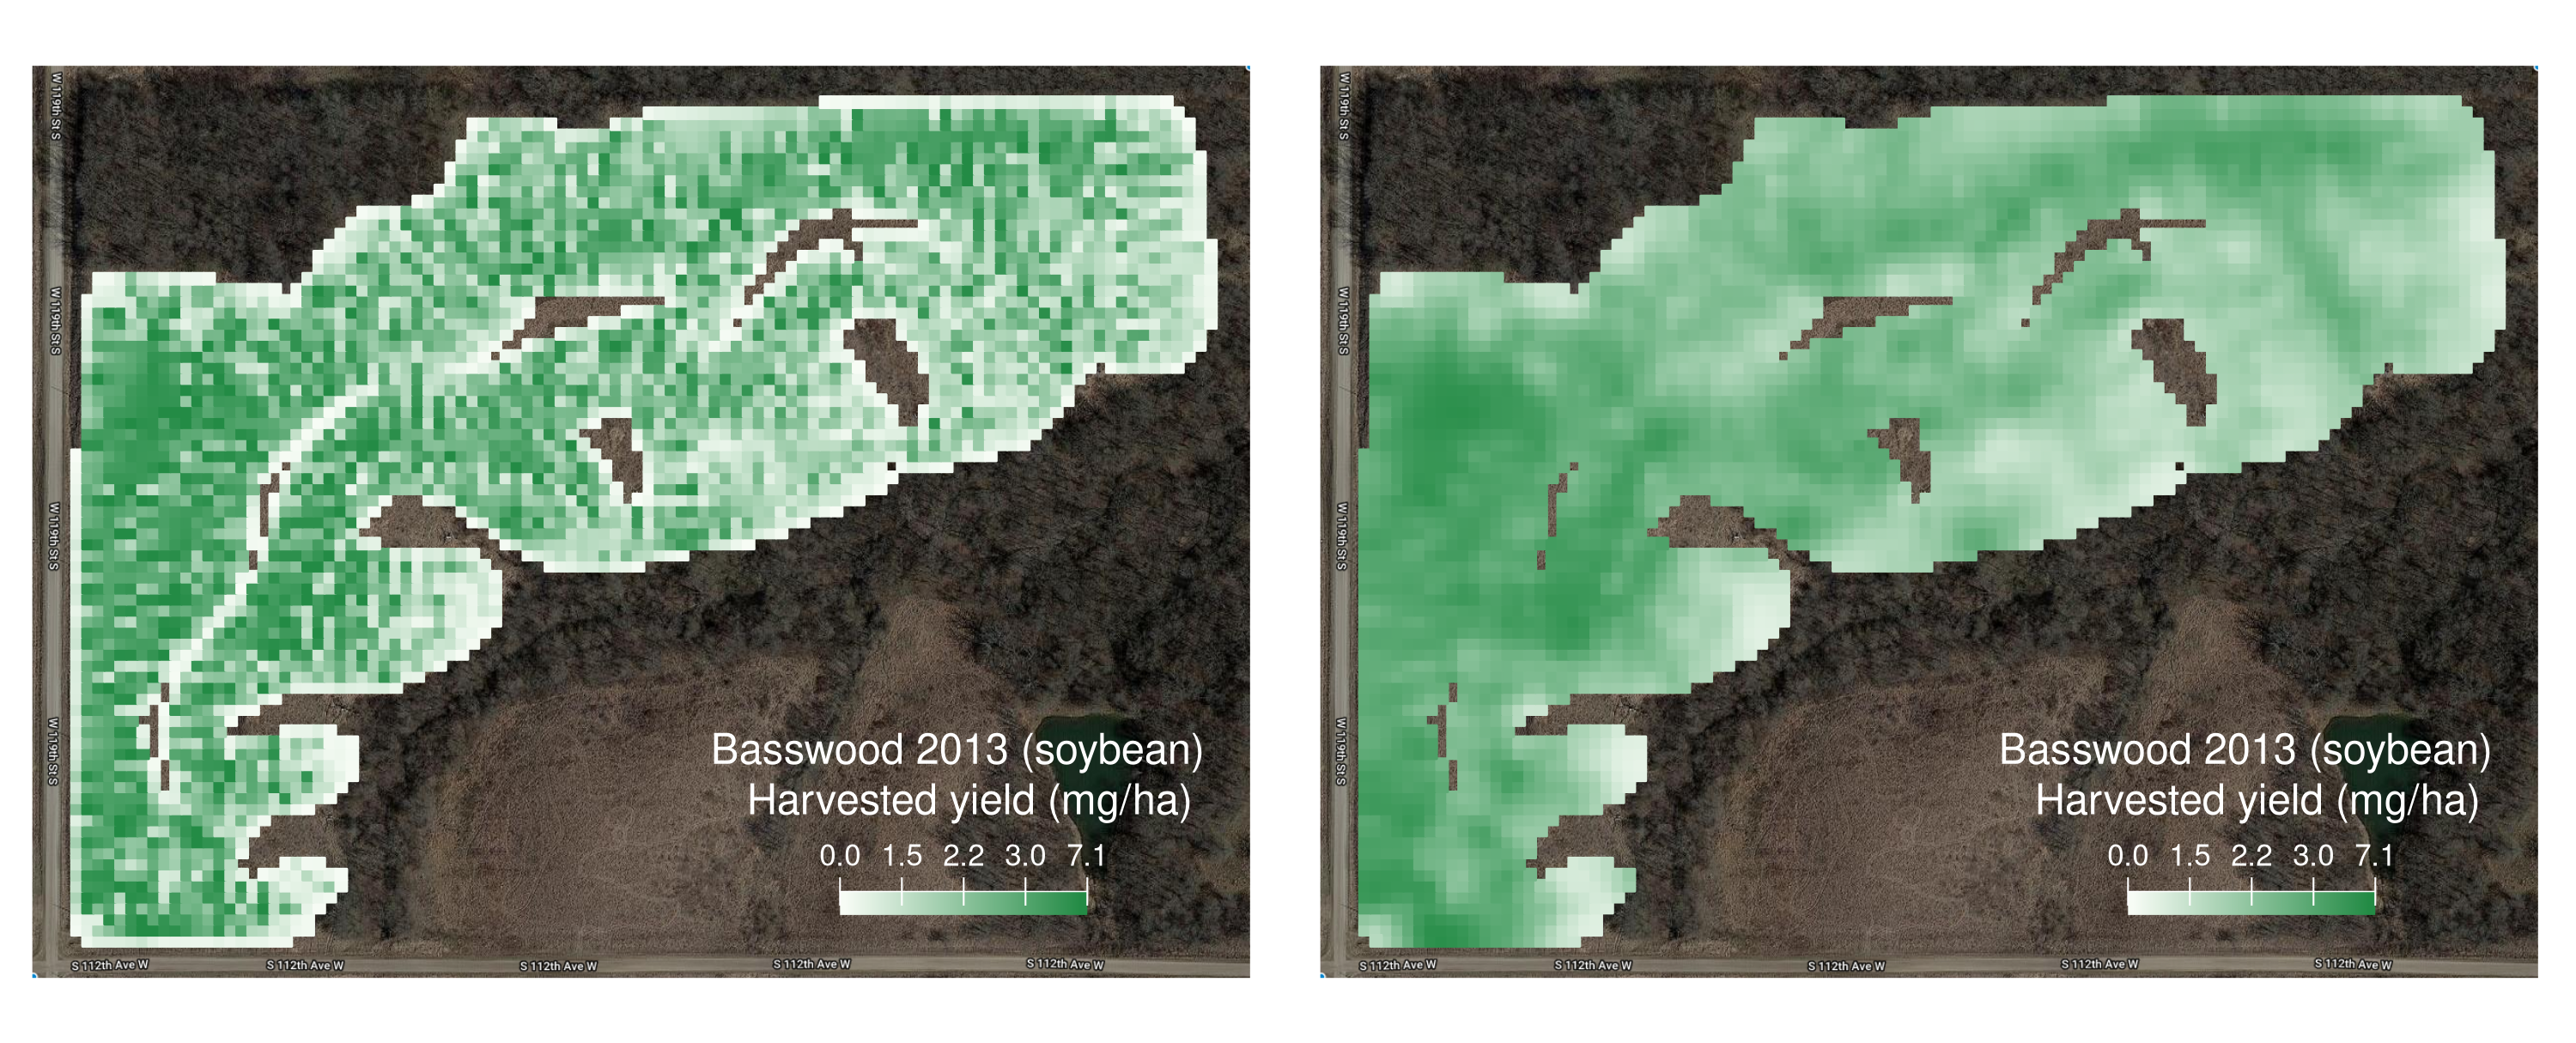
\includegraphics[width=0.95\textwidth]{./figures/maps/basswood_2013_07_gallery_res5_5.png}
  
\end{frame}

\begin{frame}
  \frametitle{Improvement quantification}

  % How to quantify the improvement in terms of ``variance reduction''
  % What's behind the fancy plots?
  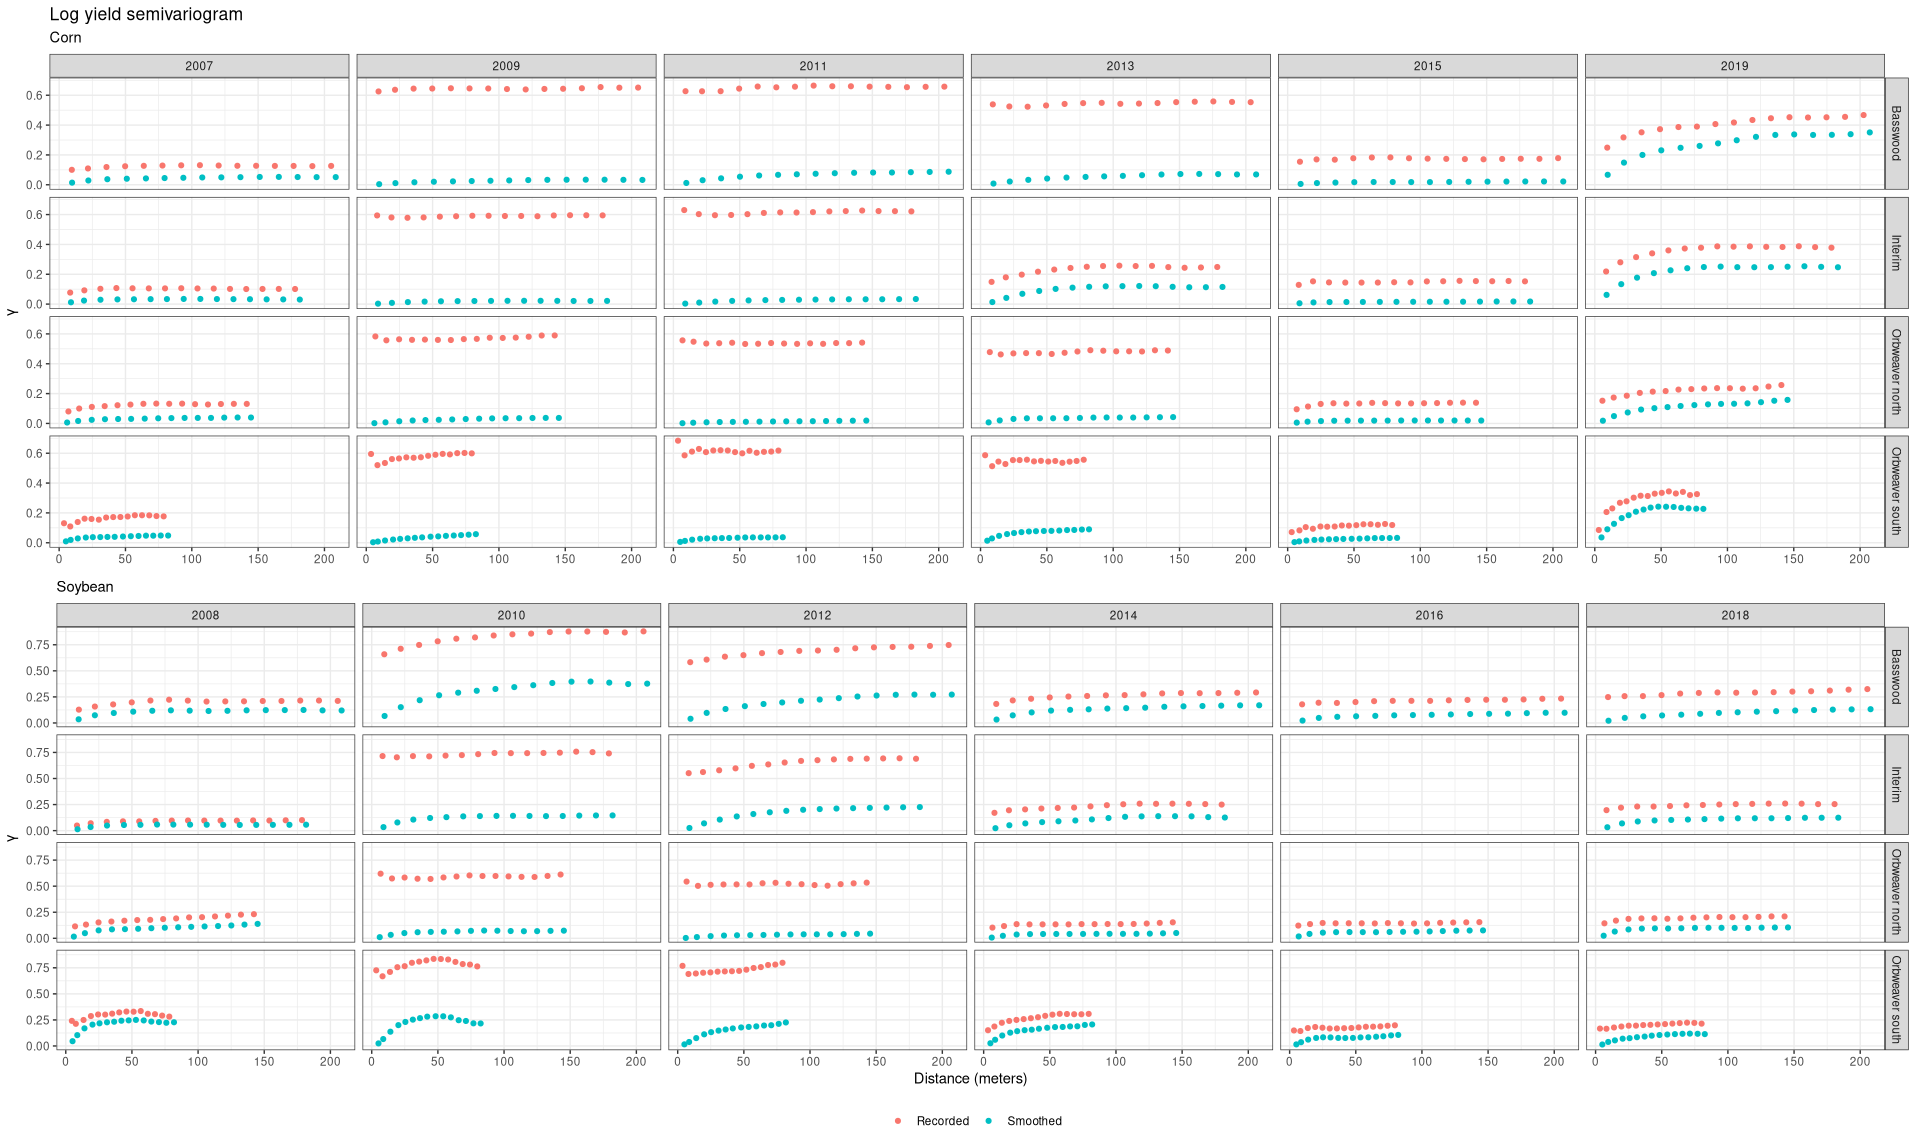
\includegraphics[width=0.95\textwidth]{./figures/semivariograms.png}

\end{frame}

\begin{frame}
  \frametitle{Resolution selection}

  \scriptsize{9x9m} \includegraphics[width=0.4\textwidth]{./figures/maps/basswood_2012_06_smoothed_res9_9.png}
  \scriptsize{7x7m} 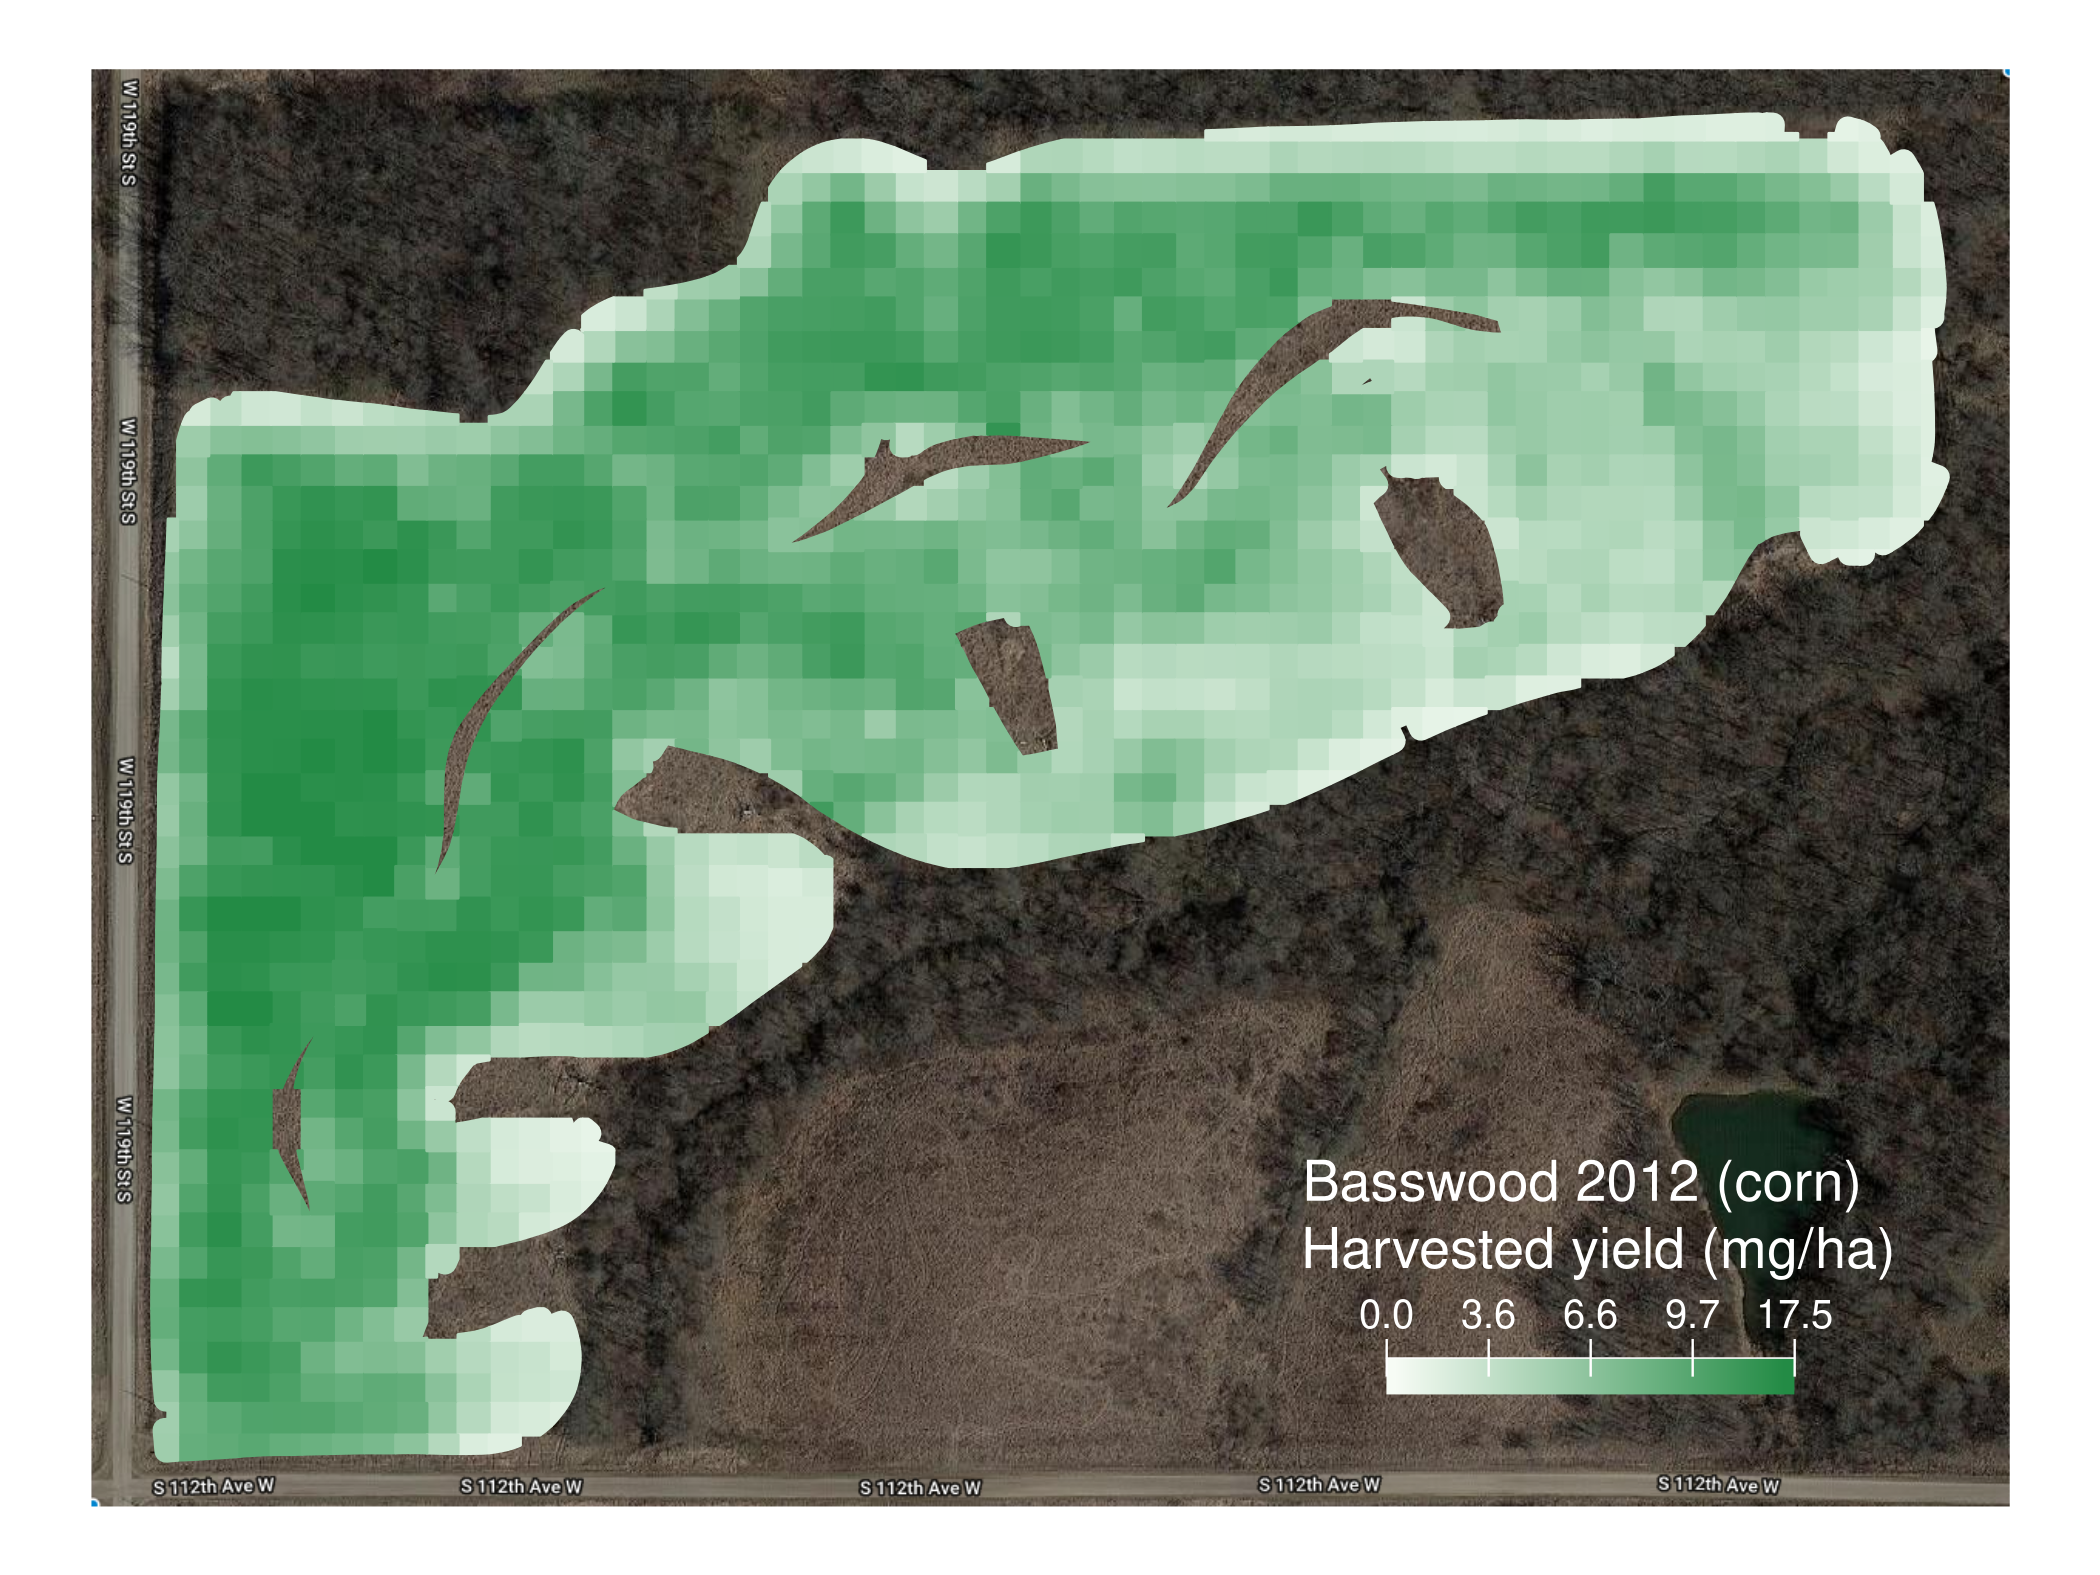
\includegraphics[width=0.4\textwidth]{./figures/maps/basswood_2012_06_smoothed_res7_7.png}

  \vspace{10px}
  \hrule
  \scriptsize{5x5m} 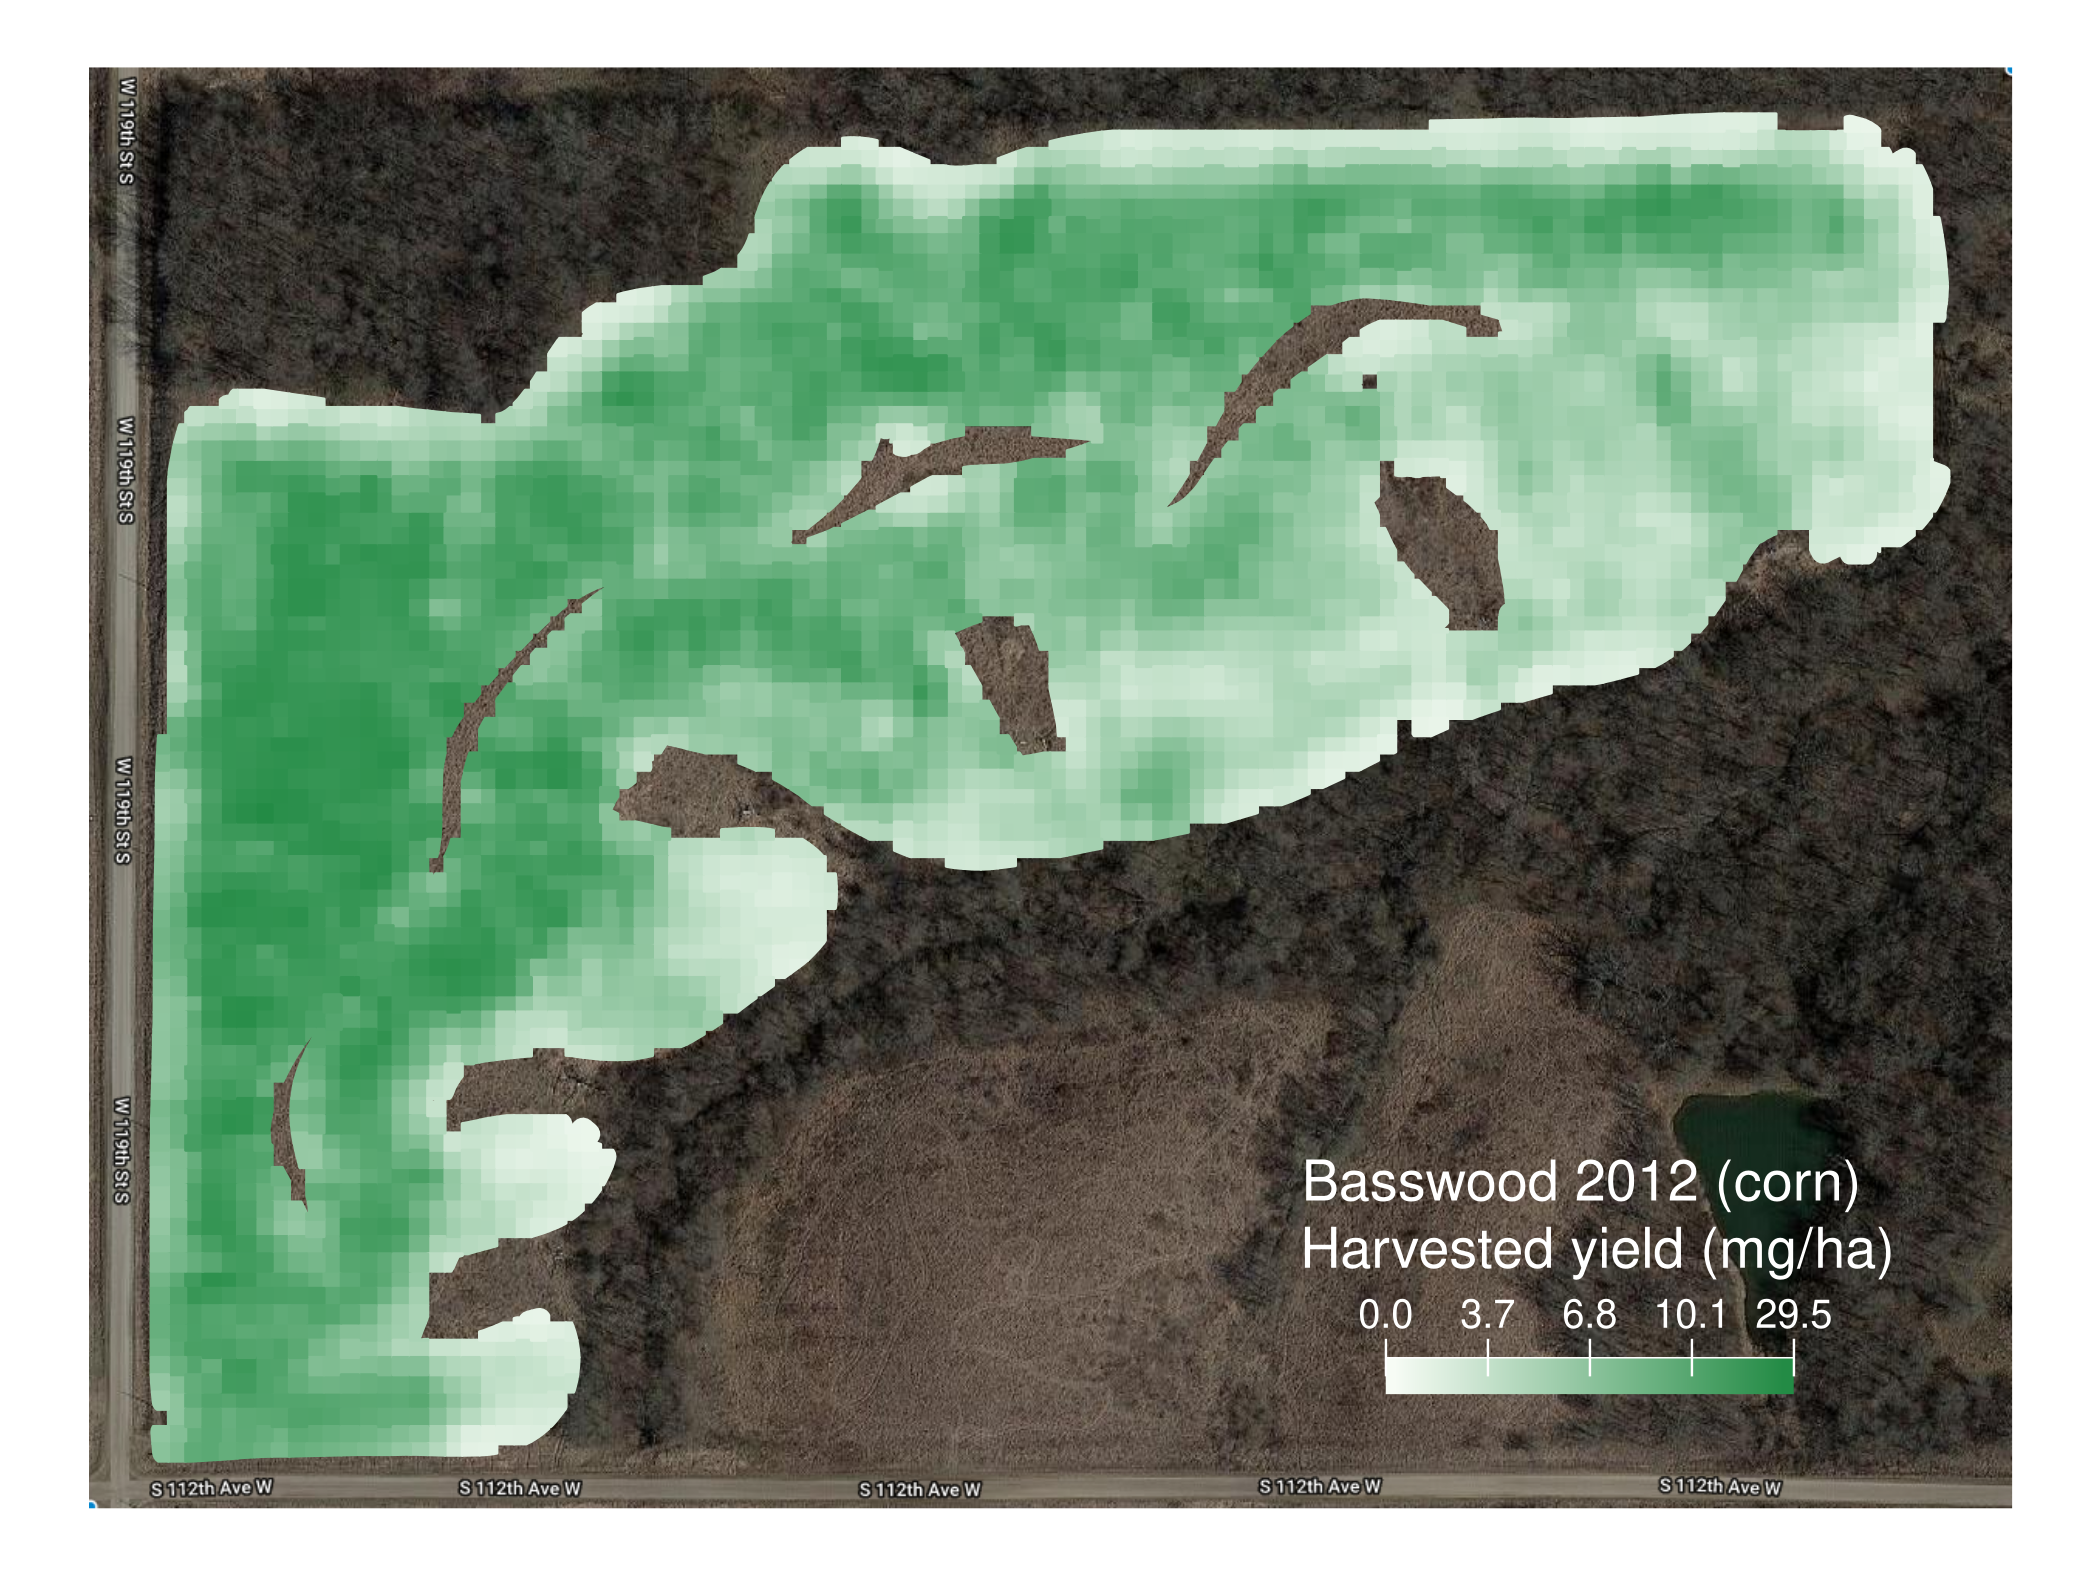
\includegraphics[width=0.4\textwidth]{./figures/maps/basswood_2012_06_smoothed_res5_5.png}
  \scriptsize{3x3m} 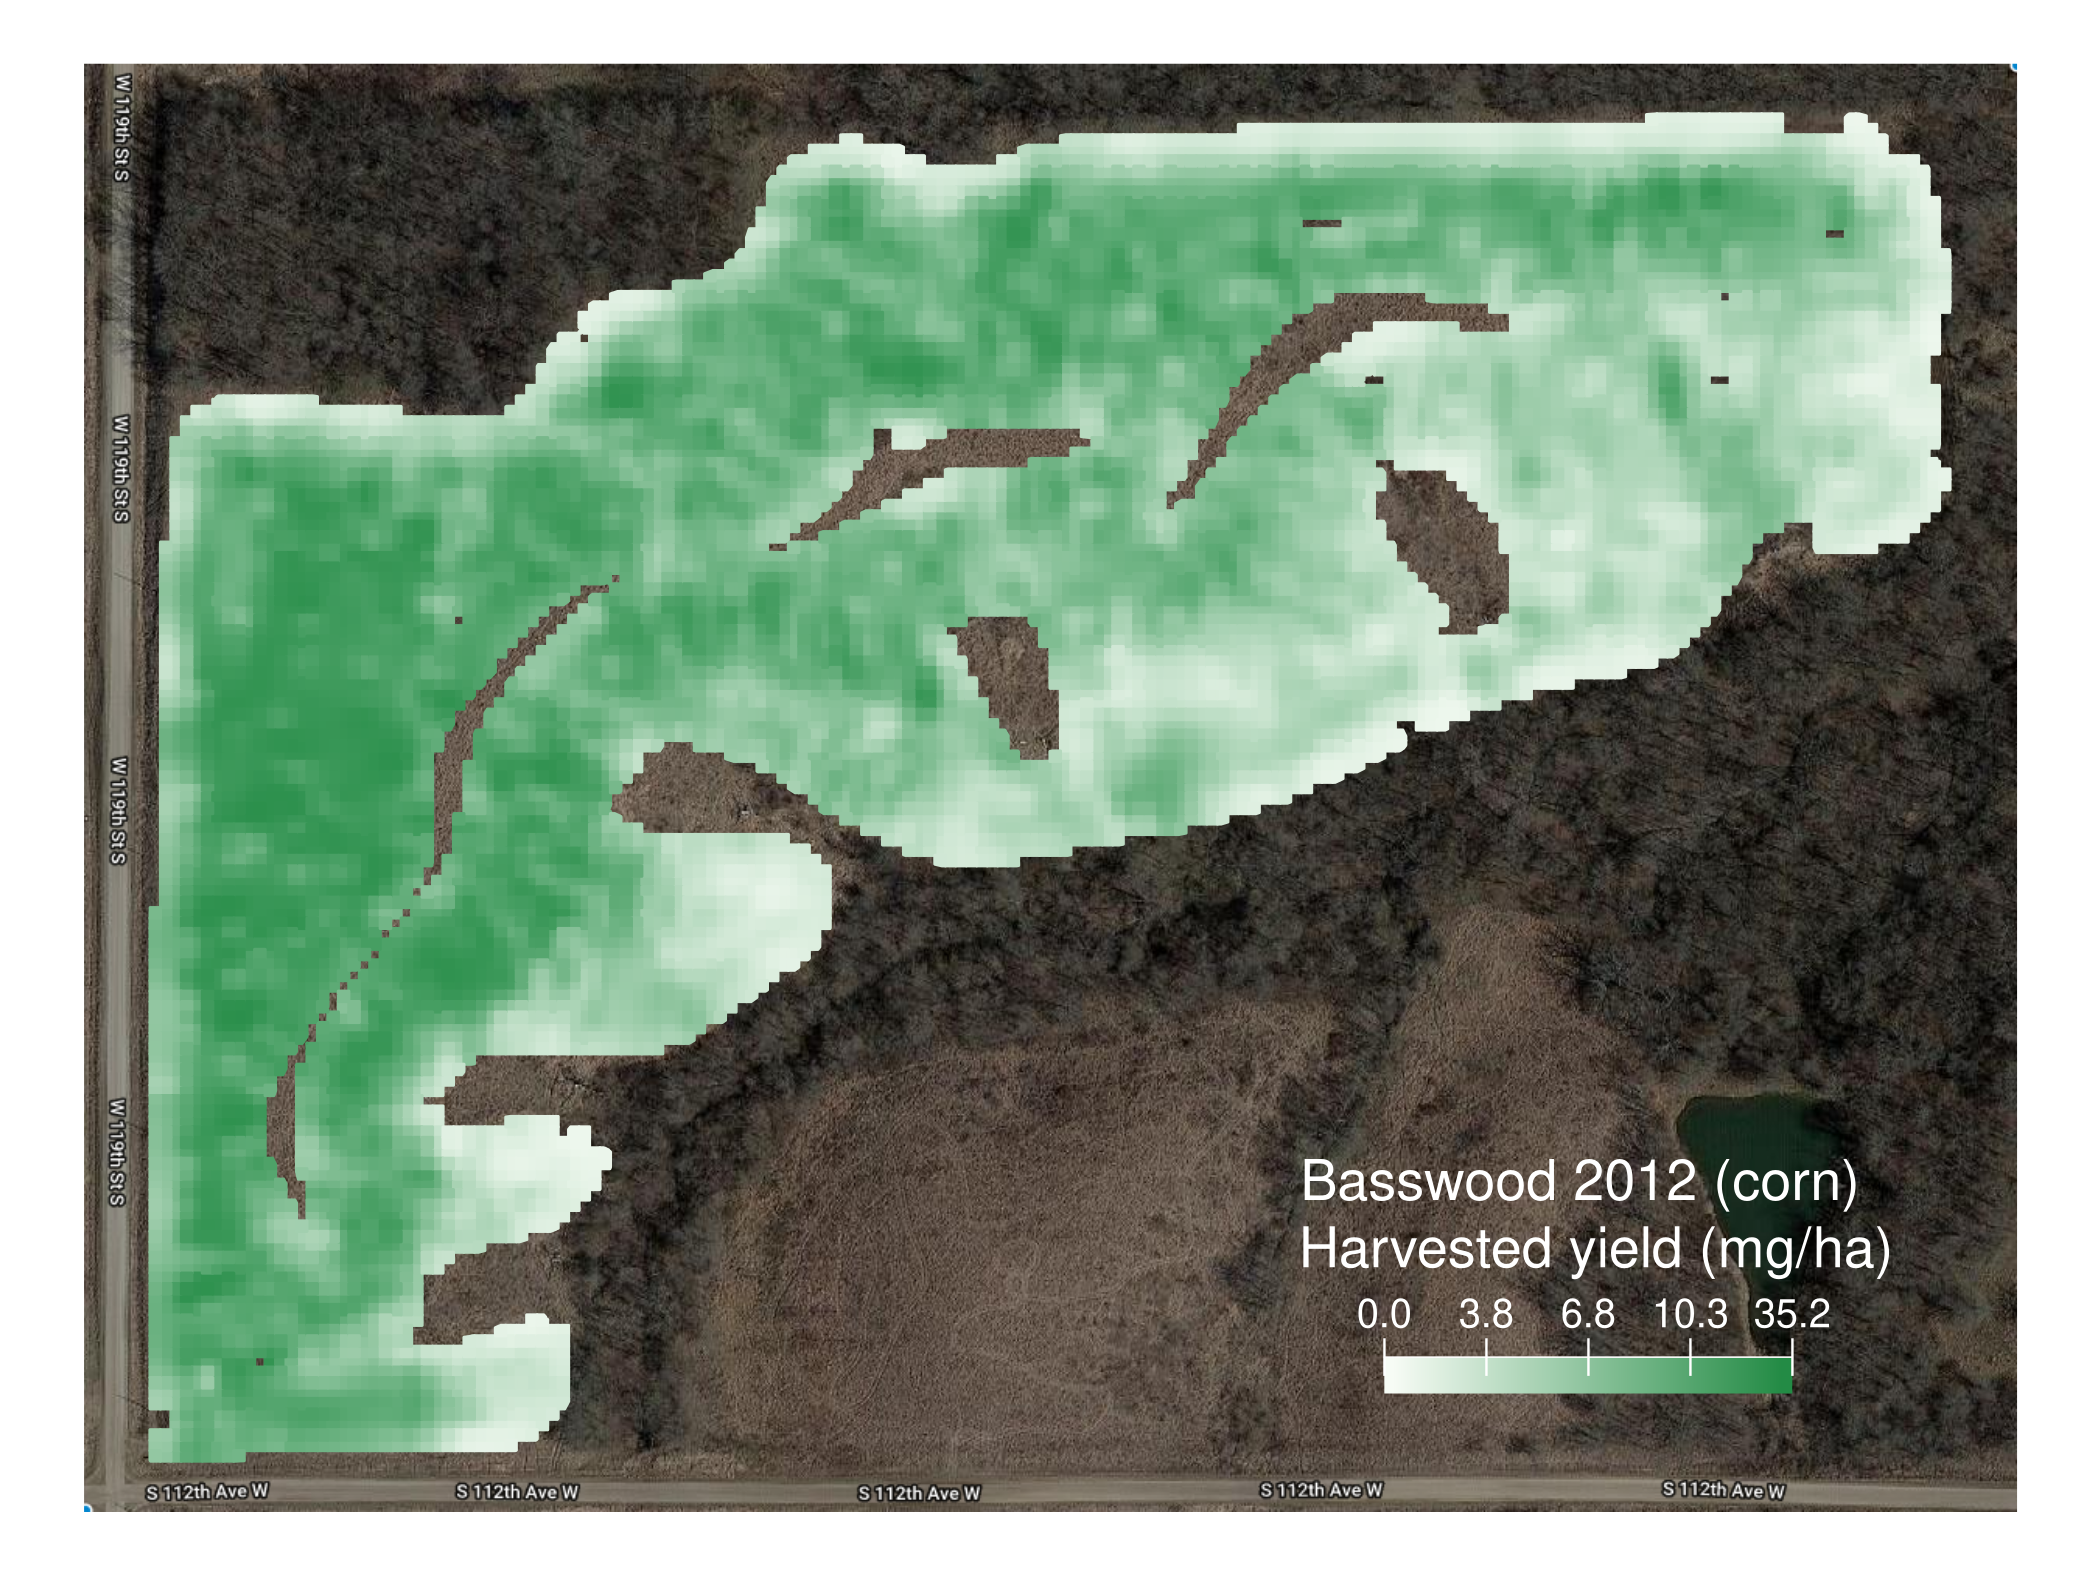
\includegraphics[width=0.4\textwidth]{./figures/maps/basswood_2012_06_smoothed_res3_3.png}
  
  % Show maps at different resolutions: aggregate, 10, 7, 5,
  % 3. Overfits?
  % Resolution selection
  % Why does the map deteriorate?
  
\end{frame}

%%%%%%%%%%%%%%%%%%%%%%%%%%%%%%%%%%%%%%%%%%%%%%%%%%%%%%%%%%%%%%%%%%%%%%%%%%
% References                                                             %
%%%%%%%%%%%%%%%%%%%%%%%%%%%%%%%%%%%%%%%%%%%%%%%%%%%%%%%%%%%%%%%%%%%%%%%%%%

\section{References}

\begin{frame}
  \frametitle{References}

  % References
  
\end{frame}

\end{document}
%%% Local Variables:
%%% mode: latex
%%% TeX-master: t
%%% End:
